\documentclass[10pt]{article}

\usepackage{times}
\usepackage{mathptmx}
\usepackage{amsmath}
\usepackage{mathtools}
\usepackage{graphicx}
\usepackage{epstopdf}

\setlength\parindent{0pt}


\raggedbottom
\sloppy

\title{Time-discrete Stochastic Signals\\
\emph{TSDT14}}

\author{David Habrman \\ davha227, 920908-2412\\
Jens Edhammer \\ jened502, 920128-5112 }

\date{\today}

\begin{document}

\maketitle

\section{Introduction}
This is a laboration report in signal theory (TSDT14). It consists of three studies.

\subsection{Study 1 – Modelling Signals}
Study 1 involves analyzing the power spectral density (PSD) and auto correlation function (ACF)
of noise filtered through two diffrent filters. One close to ideal and one simple low pass filter.
The ACF and PSD were first theoretically calculated and then estimated.
The ACF was estimated using Blackman-Tukey's- and Barlett's -estimate and the
PDF was estimated using periodograms, averaged periodograms and smoothed periodograms.

\subsection{Notation}
The following notations will be used. \\
PSD - Power Spectral Density \\
ACF - Auto correlation function \\
$\hat{r_y}$ - Estimated ACF of signal y. \\
$\hat{R_y}$ - Estimated PSD of signal y. \\
WGN - White Gaussian Noise

\section{Method}
\subsection{Study 1 – Modelling Signals}

White Gaussian noise is used in this study. It was filtered through the two
 filters described in equation~\ref{eq:simpleH} and equation~\ref{eq:idealH},
  to produce our signal y.
 The ideal filter is approximated by a highorder Butterworth lowpass filter.

\begin{equation}
  \label{eq:simpleH}
  H[\theta]_{simple} =\frac{1-a}{1-ae^{-j2\pi\theta }}
\end{equation}

\begin{equation}
  \label{eq:idealH}
  H[\theta]_{ideal} =rect(\frac{\theta}{\theta_0} )
\end{equation}

\subsubsection{Theoretical ACF and PSD}
PSD of WGN is constant and our WGN has a variance of one. Due to this the PSD
of our noise, $R_x$, is chosen to one.
The PSD of the filtered WGN is then calculated using equation~\ref{eq:PSDformula}.

\begin{equation}
  \label{eq:PSDformula}
  R_y[\theta] = R_x|H(\theta)|^2;
\end{equation}

The ACF can be calculated using inverse fourier transform, see equation~\ref{eq:ACFformula}

\begin{equation}
  \label{eq:ACFformula}
  r_y[n] = \mathcal{F}^{-1}\{R_y\}[n]
\end{equation}



\subsubsection{Estimated ACF and PSD}
The ACF was to be estimated using Blackman-Tukey's- and Barlett's -estimate.
This was done using equation~\ref{eq:BmanT} and equation ~\ref{eq:Blett}.

\begin{equation}
\label{eq:BmanT}
\hat{r}_y[k] =
\begin{cases}
    \frac{1}{N-|k|}\sum_{n=0}^{N-|k|-1}r_x[n+|k|]r_x[n],& \text{if } |k|< N\\
    0,              & \text{elsewhere}
\end{cases}
\end{equation}


\begin{equation}
\label{eq:Blett}
\hat{r}_y[k] =
\begin{cases}
    \frac{1}{N}\sum_{n=0}^{N-|k|-1}r_x[n+|k|]r_x[n],& \text{if } |k|< N\\
    0,              & \text{elsewhere}
\end{cases}
\end{equation}

The PSD was estimated using periodograms, averaged periodograms
and smoothing. The raw periodogram was calculated by taking the fouriertransform
of the estimated ACF.
Averaged periodograms was done by calculating a mean of the periodogram inside
an interval and repeating this for all samples. The averaged periodogram was
then set to the mean inside each interval.

The smoothed periodogram was done by first multiplying the estimated ACF with a
 suitable window and then using the fourier transform to get the estimated PSD,
 see equation~\ref{eq:win}. This can be viewed as a form of moving average in the fourier-domain.

 \begin{equation}
 \label{eq:win}
 \hat{R}_{y,smoothed} = \mathcal{F}\{\hat{r}_yw[k]\}
 \end{equation}


\section{Result and conclusion}
\subsection{Study 1 – Modelling Signals}

Noted in equation~\ref{eq:ACFsimple} is the theoretically calculated functions for the ACF
for the simple filter and equation~\ref{eq:ACFideal} for the close to ideal filter.
Equation~\ref{eq:PSDsimple} does the same for the simple filter's PSD
and equation~\ref{eq:PSDideal}, the close to ideal filter's PSD.

\begin{equation}
  \label{eq:ACFsimple}
  r_{y,simple} = R_x\frac{(1-a)}{(1+a)}a^{|n|};  |a| < 1
\end{equation}

\begin{equation}
  \label{eq:PSDsimple}
  R_{y,simple} =  R_x|\frac{1-a}{1-ae^{-j2\pi\theta}}|^2;
\end{equation}

\begin{equation}
  \label{eq:ACFideal}
  r_{y,ideal} = R_x\theta_{0}sinc(n\theta_0);
\end{equation}

\begin{equation}
  \label{eq:PSDideal}
  R_{y,ideal} = R_xrect(\frac{\theta - k}{\theta_0})
\end{equation}


The theoretical functions for the ACF and PSD for $y_{simple}$ are presented
in figure~\ref{fig:TheoACFsimple} and figure~\ref{fig:TheoPSDsimple}
The functions for $y_{ideal}$ are presented in figure~\ref{fig:TheoACFideal} and
figure~\ref{fig:TheoPSDideal}



\begin{figure}[!hp]

    \begin{center}
      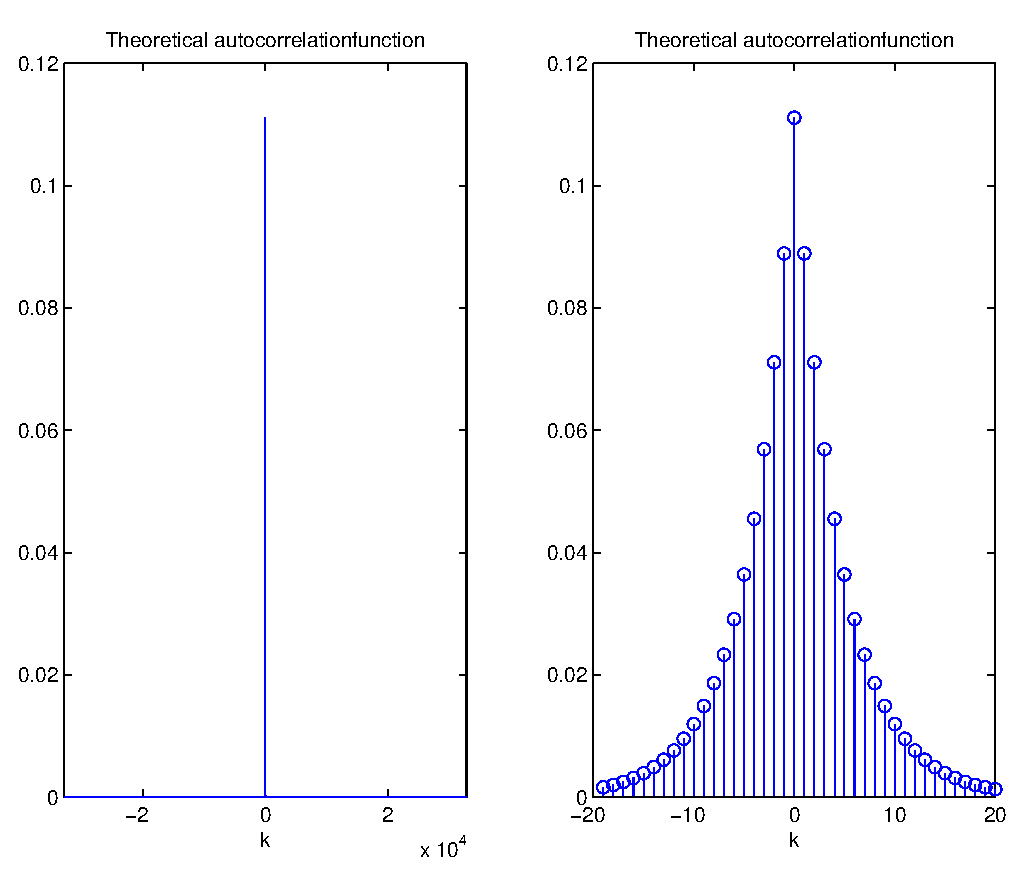
\includegraphics[width=0.6\textwidth]{TheoACF}
    \caption{Theoretical ACF of $y_{simple}$ \label{fig:TheoACFsimple}}
    \end{center}

\end{figure}

\begin{figure}[!hp]

    \begin{center}
      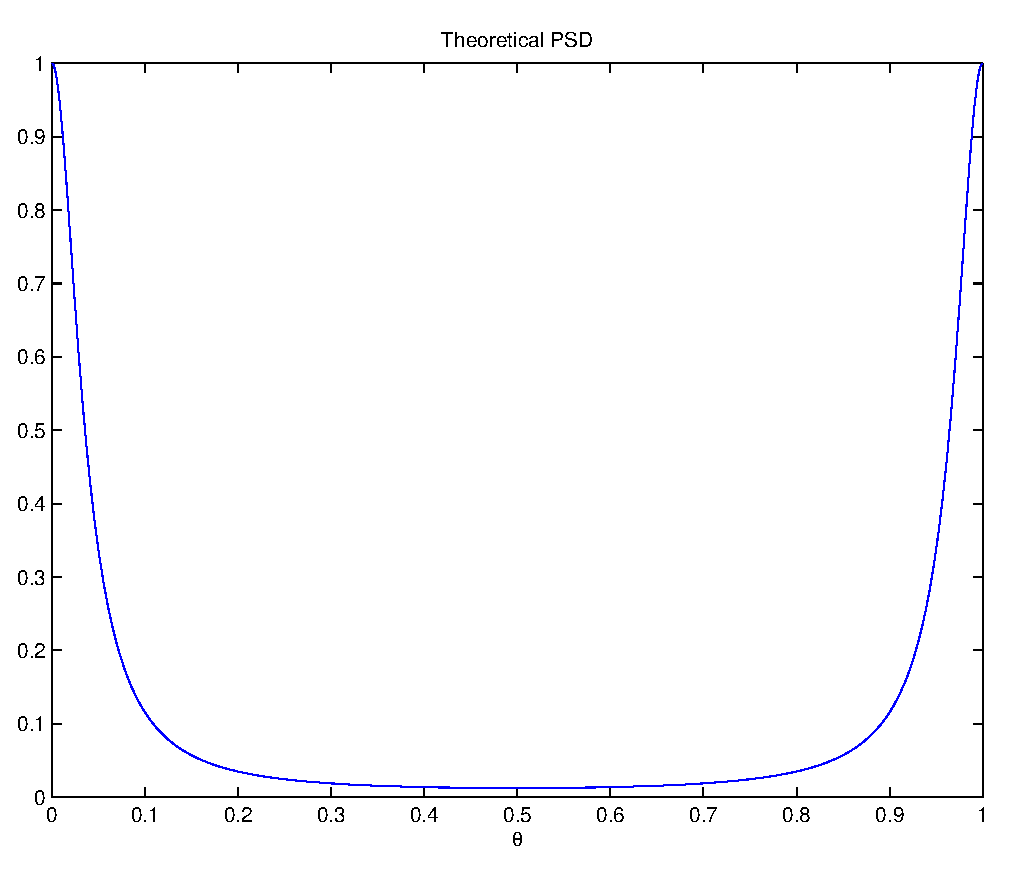
\includegraphics[width=0.6\textwidth]{TheoPSD}
    \caption{Theoretical PSD of $y_{simple}$ \label{fig:TheoPSDsimple}}
    \end{center}

\end{figure}

\begin{figure}[!hp]

    \begin{center}
      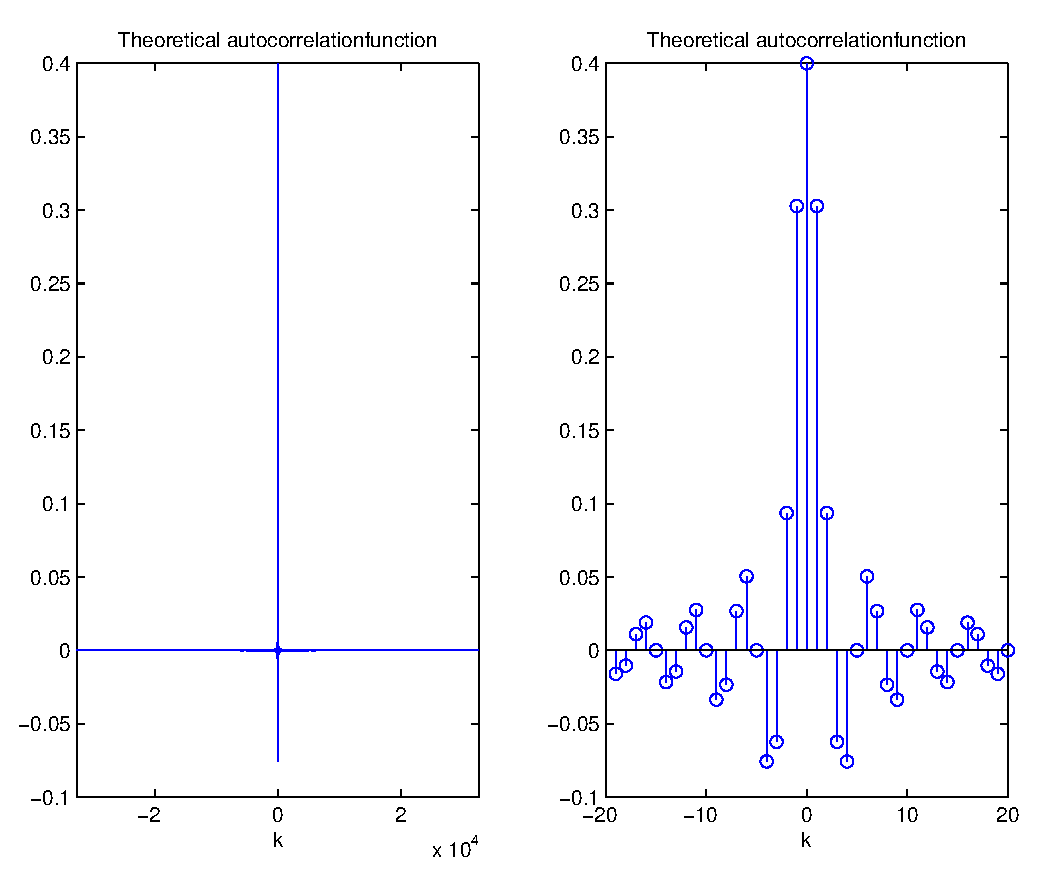
\includegraphics[width=0.6\textwidth]{BTheoACF}
    \caption{Theoretical ACF of $y_{ideal}$ \label{fig:TheoACFideal}}

    \end{center}

\end{figure}

\begin{figure}[!hp]

    \begin{center}
      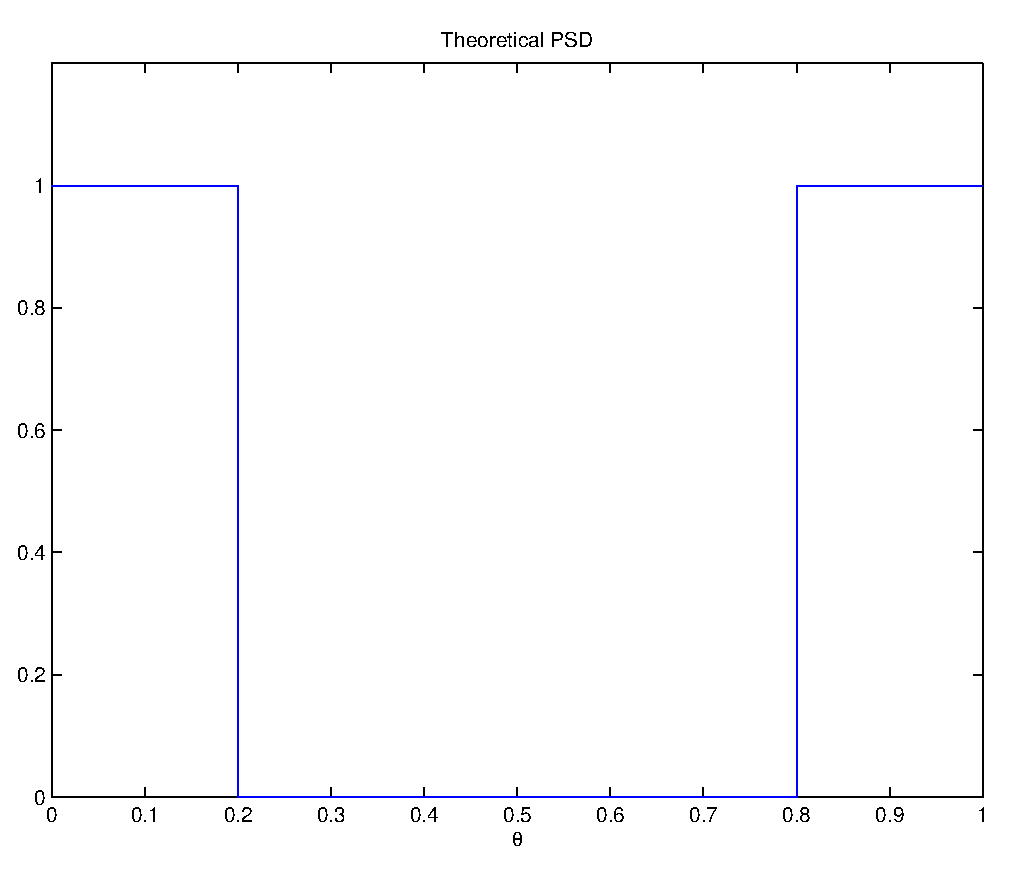
\includegraphics[width=0.6\textwidth]{BTheoPSD}
    \caption{Theoretical PSD of $y_{ideal}$ \label{fig:TheoPSDideal}}
    \end{center}

\end{figure}

\clearpage

\subsubsection{ACF estimation}

ACF estimations, of the signal filtered through the simple filter, using Blackman-
Turkey’s and Barlett’s-estimate are shown in figure~\ref{fig:ACFest}. The estimations of the signal
filtered through the near ideal filter are shown in figure~\ref{fig:BACFest}.
By examining the pictures you see the difference between the theoretical ACF and
the estimated ACF for both filters. The theoretical ACF tends to zero for higher k
while both Blackman-Turkey’s and Barlett’s-estimate are non-zero for higher k. This is
due to the fact that both Blackman-Turkey’s and Barlett’s-estimate have variances not
tending to zero for higher k. You can also see that Barlett’s estimate is slightly better
than Blackman-Turkey’s. \\


\begin{figure}[!hp]

    \begin{center}
      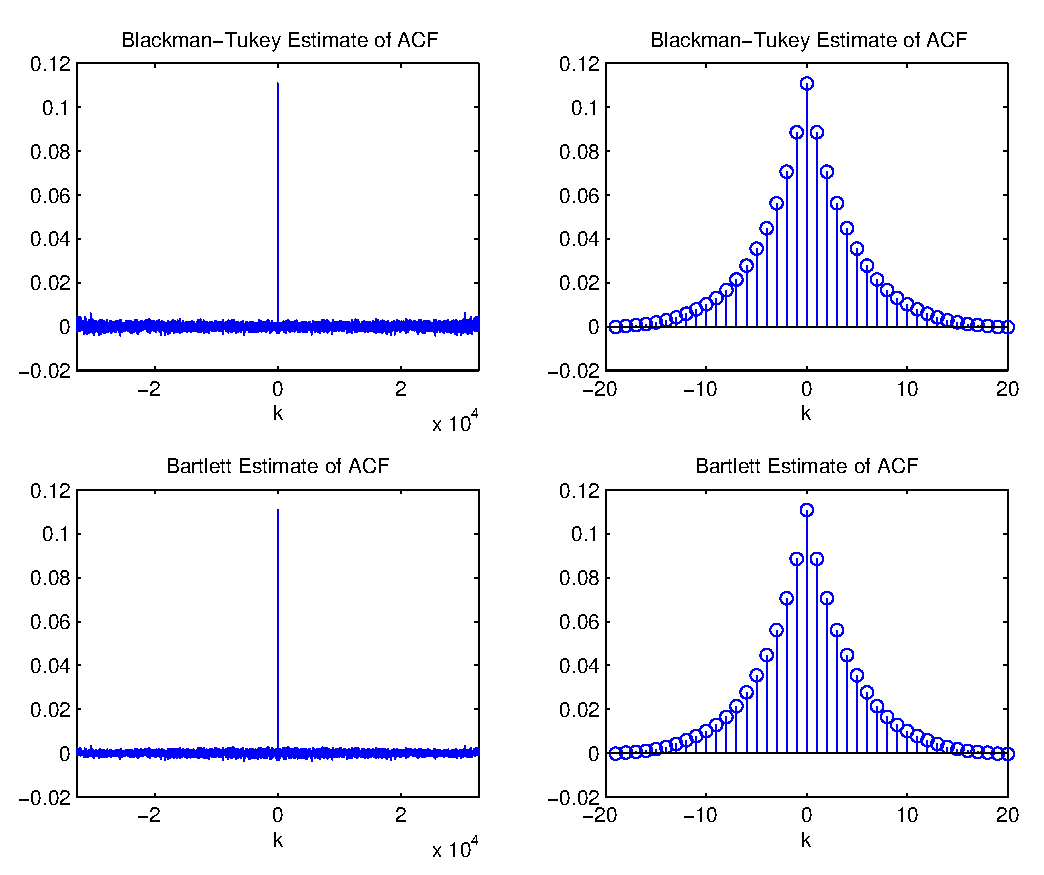
\includegraphics[width=0.6\textwidth]{EstACF}
    \caption{Estimated ACF of $y_{simple}$ \label{fig:ACFest}}
    \end{center}

\end{figure}

\begin{figure}[!hp]

    \begin{center}
      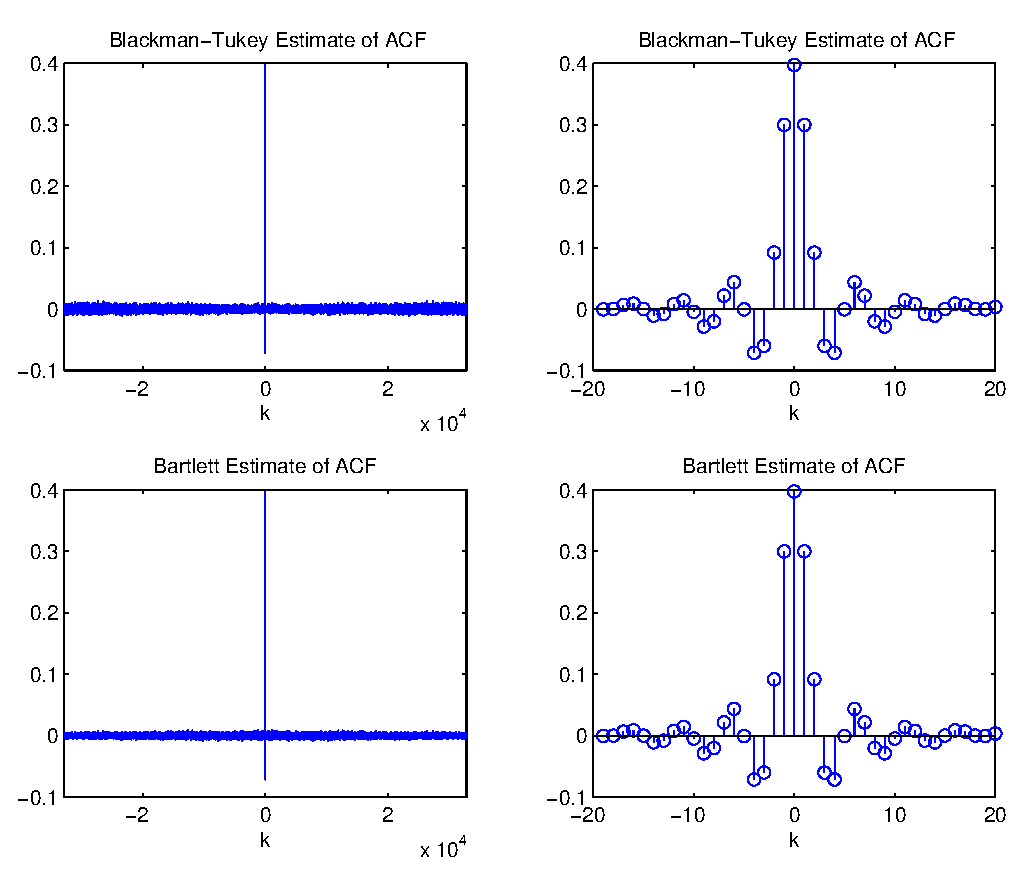
\includegraphics[width=0.6\textwidth]{BEstACF}
    \caption{Estimated ACF of $y_{ideal}$ \label{fig:BACFest}}
    \end{center}

\end{figure}

\clearpage

\subsubsection{PSD estimation}


PSD estimations of the signal filtered through the simple filter are
shown in figure~\ref{fig:PSDest} and figure~\ref{fig:PSDSmooth} while the estimations of the signal
filtered through the near ideal filter are shown in figure~\ref{fig:BPSDest} and
figure~\ref{fig:BPSDSmooth}. The raw periodogram follows the shape of the theoretical
PSD but it has a large variance. This variance was improved when using averaged periodogram,
 as can be seen in figure~\ref{fig:PSDest} and figure~\ref{fig:BPSDest}.
 However, this method sacrifices frequency resolution for a smaller variance.
 When using smoothed periodogram the variance was small and no frequency
 resolution sacrifices had to be made.


\begin{figure}[!hp]

    \begin{center}
      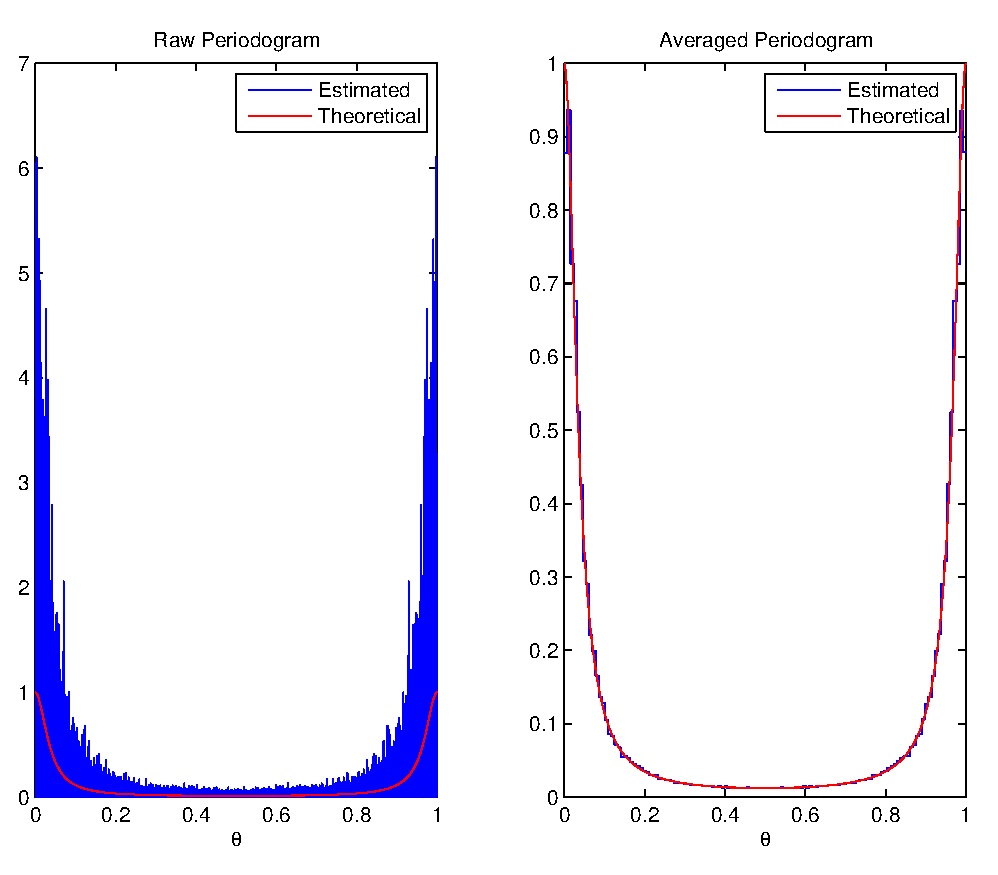
\includegraphics[width=0.6\textwidth]{Periodogram}
    \caption{Estimate PSD of $y_{simple}$ \label{fig:PSDest}}
    \end{center}

\end{figure}

\begin{figure}[!hp]

    \begin{center}
      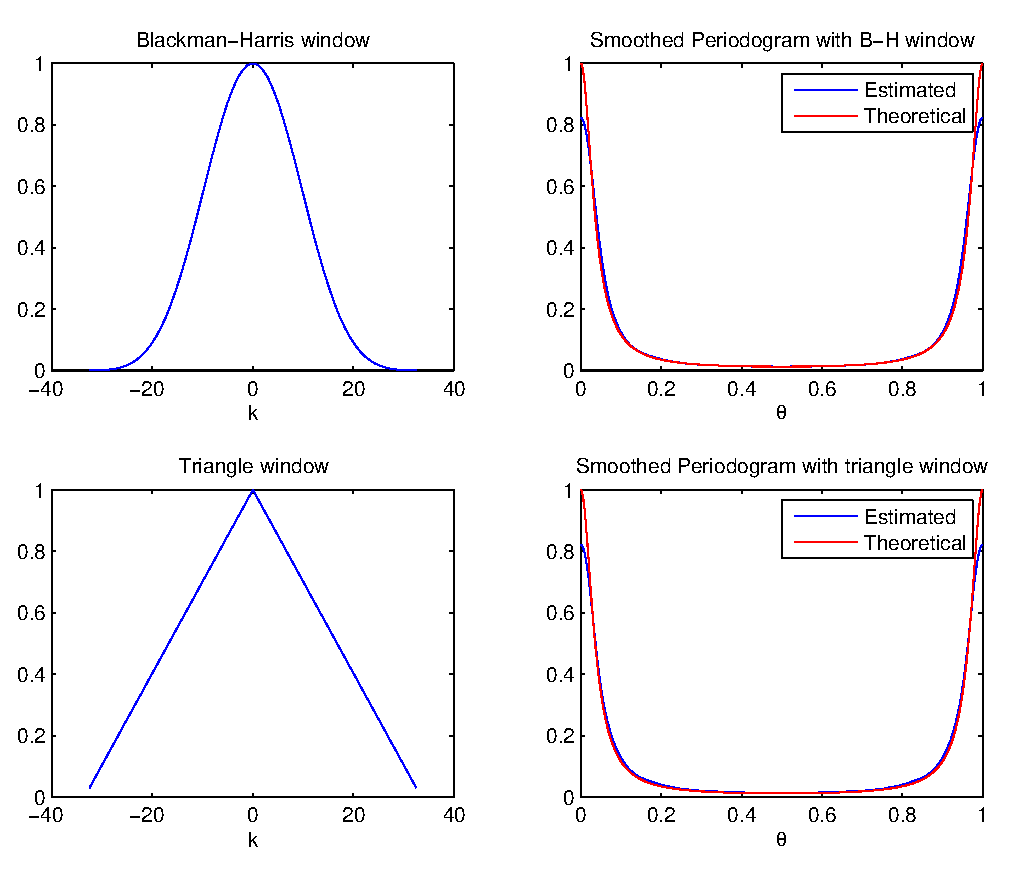
\includegraphics[width=0.6\textwidth]{Smoothed}
    \caption{Smoothed PSD of $y_{simple}$ \label{fig:PSDSmooth}}
    \end{center}

\end{figure}

\begin{figure}[!hp]

    \begin{center}
      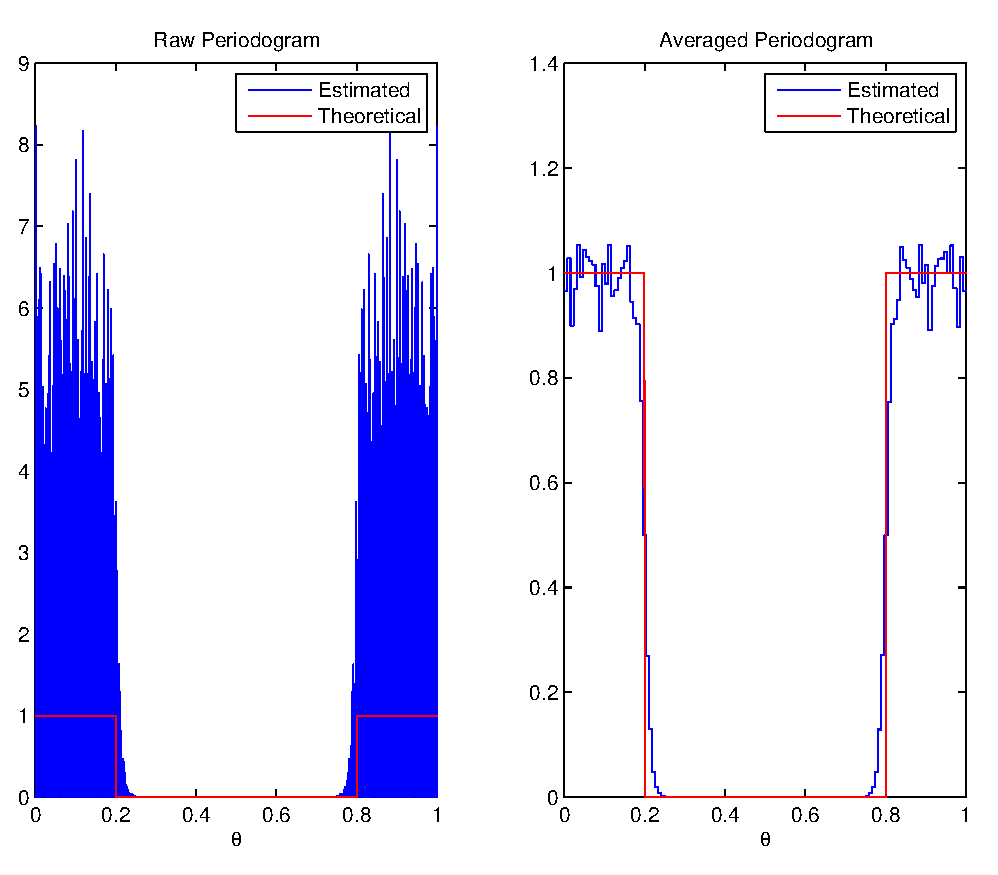
\includegraphics[width=0.6\textwidth]{BPeriodogram}
    \caption{Estimate PSD of $y_{ideal}$ \label{fig:BPSDest}}
    \end{center}

\end{figure}

\begin{figure}[!hp]

    \begin{center}
      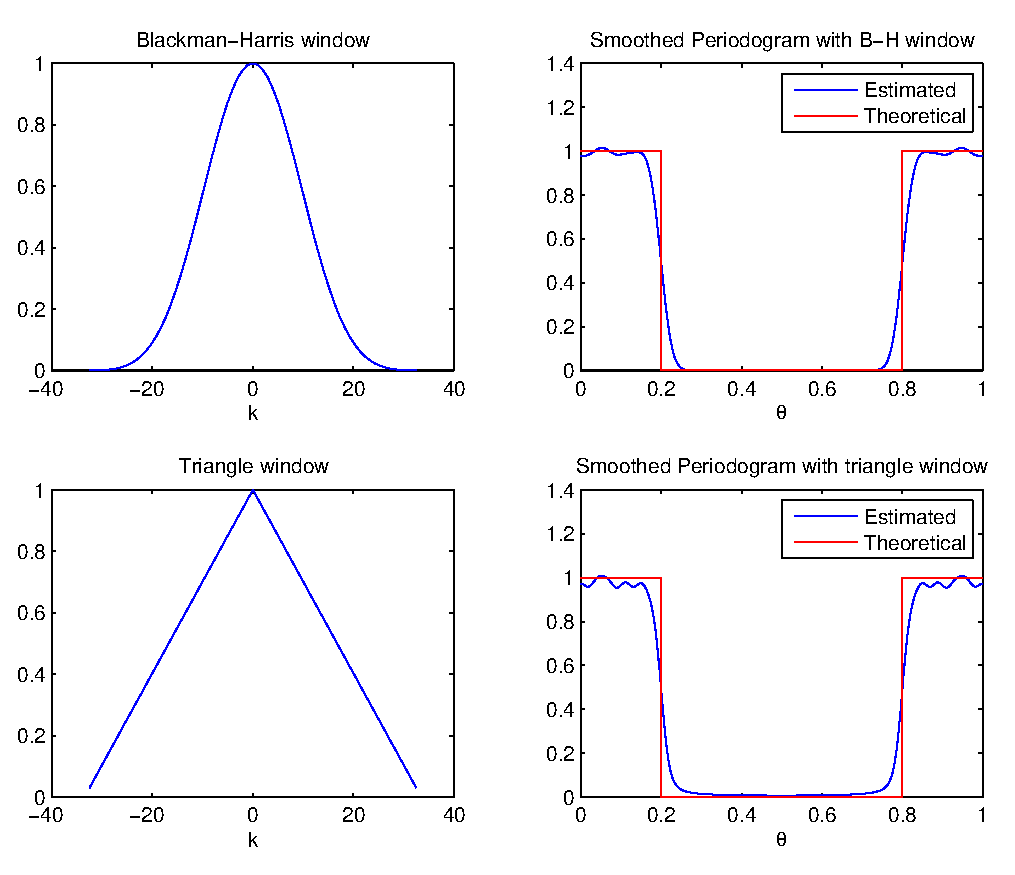
\includegraphics[width=0.6\textwidth]{BSmoothed}
    \caption{Smoothed PSD of $y_{ideal}$ \label{fig:BPSDSmooth}}
    \end{center}

\end{figure}




\clearpage

\end{document}
